\documentclass[conference]{IEEEtran}

\usepackage{graphicx}
\usepackage{url}

\newcommand{\todo}[1]{ \textbf{#1} }
\newcommand{\quotes}[1]{\textit{``#1''}}

% correct bad hyphenation here
\hyphenation{op-tical net-works semi-conduc-tor}


\begin{document}

\title{How do Scratch Users Name Variables and Functions? }

% author names and affiliations
% use a multiple column layout for up to three different
% affiliations
\author{\IEEEauthorblockN{Author1}
\IEEEauthorblockA{Uni1\\
Address1\\
Email: email1.com}
\and
\IEEEauthorblockN{Author2}
\IEEEauthorblockA{Uni2\\
	Address2\\
	Email: email2.com}}
% make the title area
\maketitle

% As a general rule, do not put math, special symbols or citations
% in the abstract
\begin{abstract}
The abstract goes here.
\end{abstract}

\IEEEpeerreviewmaketitle



\section{Introduction}
The naming of identifiers in software code is considered, by several researchers, as one important aspect of its quality~\cite{AmanASK15,AnquetilL98,AvidanF17,Beniamini,ButlerWYS10,CaprileT00,HofmeisterSH17,LawrieMFB07,LunguK13,ScannielloR13,TakangGM96,TramontanaRS14}. Previous studies have shown a correlation between the proper naming of identifiers and the readability and comprehension of the code.\todo{AS says: this is controversial since Beniamini~\cite{Beniamini} and Hofmeister~\cite{HofmeisterSH17} seem to disagree on this point.} Comprehension is linked to maintainability tasks and efficient performance of developers while performing them. \todo{AS says: we need either a citation to support this claim or rephrase} As one scientist once said \quotes{the code should be considered for human and less occasionally for a computer to execute}.\todo{AS asks: who has said this? This is a common adagio but I have no idea who is the author.}

Computer science and programming education seem to focus on the programming concepts and the syntax of the languages as opposed to practices in naming variables and identifiers. 
Indeed, neither the ACM Curriculum Guidelines for Undergraduate Programs in Computer Science\footnote{\url{http://www.acm.org/education/CS2013-final-report.pdf}} nor the Curriculum Guidelines for Undergraduate Degree Programs in Software Engineering\footnote{\url{http://www.acm.org/binaries/content/assets/education/se2014.pdf}} discuss this topic.
One of the most common examples in many programming languages is the use of \quotes{foo} and \quotes{bar} naming for variables and functions. 
These two identifiers have meaningless names, and to some extent, they represent a refusal to name, which give the learner the conception that the name is less important, or irrelevant, to the programming task. 

Recent studies have focused on the analysis of naming in software code repositories. In this paper, we give attention to novice programmers with the Scratch visual language. 
When it comes to novice programmer and learners, it is more important for the software community to understand conceptions in naming that are prevalent. These users will be the future developers, and at some point, they need to follow an implicit or explicit guideline of naming and collaborating in larger software repositories. 
To this end, we have analyzed 240,000 Scratch projects. Scratch is a block-based visual language that was developed by MIT with the aim of helping young people learn the basic concepts of programming and collaboration. Scratch has recently become very popular among school-age children and introduced as part of the curriculum in some countries as a means to teach programming. Analyzing Scratch programs will give researchers and software engineering community a perspective on naming from learners making their first step in programming and might turn to be the future programmers. In this paper we aim at answering the following research questions: \\
\begin{description}
	\item[\textbf{RQ1}] How do Scratch users name variables and procedures?
	\item[\textbf{(a)}] The length distribution of variable and function identifiers across projects.
	\item[\textbf{(b)}] The usage of single-letter variables.
	\item[\textbf{RQ2}] How do Scratch users use language-dependent features in naming identifiers? In particular, to what extent are the following usage patterns popular within Scratch projects?
	\item[\textbf{(a)}] Using spaces within identifiers
	\item[\textbf{(b)}] Using numeric digits as identifiers
	\item[\textbf{(c)}] Using the parameter in the middle name for procedures] 
	
\end{description}

\todo{More questions: analysis of the peak value of 5, what is the most recurrent name? Is it expected or justified?}
\todo{More questions: variable length based on category of the Scratch program: game animation, ....}
\todo{More questions: variable length in relation to Dr. Scratch CT}
 
\section{Background and motivation}
Naming identifiers in software code have been studied extensively in the past decades. in practice, identifiers are a major part of software code as one study found that within the Eclipse code, which has 2 MLoC, 33\% of the tokens and 72\% of characters are dedicated to identifiers. For a human to read that code, it is crucial to understand what the identifier means, and then can deduce what the code does. With no surprise, several studies have confirmed the link between good identifier naming and code's readability and comprehension. The comprehension is not a target in its own; the true reason is that better comprehension lets the developers perform maintenance tasks more effectively and efficiently.
But what is a good naming approach? It is out of this paper's scope to explore the various recommendations of good identifier naming. However, it is worth to mention that there are different perspectives on what a good name is. Some researchers emphasize the usage of actual and complete words from a dictionary, or known abbreviations, which reflect the context of the program's purpose. Others argue that consistency in naming style is the most important. The usage of single-letter identifiers attracts much attention in research. For programmers, it is tempting to choose single-letter identifiers for quicker code writing that involves less mental load on the choice of a name. Additionally, single-letter named variables such as \quotes{i} or \quotes{j} have become almost a standard choice for index values when coding loops. Research has shown however that shorter identifier names are longer to comprehend, and the length of a variable should reflect its scope. 

Despite the agreement on the importance of identifier names, and efforts to introduce naming guidelines and additional tools to help the programmer choose better names, developers find giving appropriate names to identifiers as a difficult task. In the end, it is the decision of the individual writing the code, and many factors may contribute to that decision. One area to consider here is the computer science and in particular programming education. There seems to be a great focus on the programming concepts, while less to zero attention is given to beautifying the code. For example, the usage of the identifier names \quotes{foo} and \quotes{bar} is prevalent in code examples. These names have no real meaning, and the student cannot link them to what the code does.  

We are inspired by the work done by \todo{ref} where they explored the single-letter naming for multiple software repositories from different programming languages. It is important for the software community to understand the patterns in which software developers apply naming to identifiers. We argue that this understanding can improve the quality of the guidelines and introduce research-supported tools that meet the needs of the programmers. For this sake, we believe it is even more important to focus on the novice programmers, students, and learners. For these future developers, the usage of a particular naming pattern in this level forms a (mis)conception that could move along with them to other programming languages and future careers. The work was done by \todo{add ref} excludes the visual languages which have recently become a favorable choice for elementary and high schools as an introduction to programming, for example, Scratch and Alice. These block-based languages allow the user to create and assign their identifiers for variables and blocks. By studying these identifiers, we can understand better how novice programmers apply standard and language-specific naming, and how it compares to other textual based languages previously explored in the literature. 

\section{Relevant Scratch Concepts}
\label{sec:scratch}
This paper is by no means an introduction into Scratch programming, we refer the reader to \cite{brennan_creative_2014} for an extensive overview. To make this paper self-contained, however, we explain a number of relevant concepts in this section. 

Scratch is a block-based programming language aimed at children, developed by MIT. Scratch can be used to create games and interactive animations, and is available both as a stand-alone application and as a web application. Figure \ref{fig:ui} shows the Scratch user interface in the Chrome browser.

\subsection{Sprites}
Scratch code is organized by `sprites': two-dimensional pictures each having their own associated code. Scratch allows users to bring their sprites to life in various ways, for example by moving them in the plane, having them say or think words or sentences via text balloons, but also by having them make sounds, grow, shrink and switch costumes. The Scratch program in Figure \ref{fig:ui}\footnote{\url{https://scratch.mit.edu/projects/97086781/}} consists of one sprite, the cat, which is Scratch's default sprite and logo. The code in the sprite will cause the cat to jump up, say ``hello'', and come back down, when the green flag is clicked, and to make the `meow' sound when the space bar is pressed.

\begin{figure}
  \begin{center}
  \includegraphics[width=\columnwidth]{fig/ui.png}
  \caption{The Scratch user interface consisting of the `cat' sprite on the left, the toolbox with available blocks in the category `motion' in the middle and the code associated with the sprite on the right. The upper right corner shows the actual location of the sprite.}
  \label{fig:ui}
  \end{center}
\end{figure} 

\subsection{Events}
Scratch is \emph{event-driven}: all motions, sounds and changes in the looks of sprites are initiated by events. The canonical event is the `when Green Flag clicked', activated by clicking the green flag at the top of the user interface. In addition to the green flag, there are a number of other events possible, including key presses, mouse clicks and input from a computer's microphone or webcam. In the Scratch code in Figure \ref{fig:ui} there are two events: `when Green Flag clicked' and `when space key pressed'

\subsection{Scripts}
Source code within sprites is organized in scripts: a script always starts with an event, followed by a number of blocks. The Scratch code in Figure \ref{fig:ui} has two distinct scripts, one started by clicking on the green flag and one by pressing the space bar. It is possible for a single sprite to have multiple scripts initiated by the same event. In that case, all scripts will be executed simultaneously. 

\subsection{Remixing}
Scratch programs can be shared by their creators in the global Scratch repository\footnote{\url{https://scratch.mit.edu/explore/projects/all/}}. Shared Scratch programs can be `remixed' by other Scratch users, which means that a copy of this program is placed in the user's own project collection, and can be then further changed. The `remix tree' of projects is public, so users can track which users remix their programs, a bit similar forking in GitHub. Contrary to forking however, changes upstream cannot be integrated back into the original project. Because Scratch users can remix each others programs, maintainability of programs is important. A given Scratch program can be read and adapted by many children, there are projects on the Scratch home page which are remixed hundreds of times. \todo{maybe this part about importance should be move somewhere else? this section might be skipped.}

\subsection{Variables}
Like most textual languages, Scratch users can use variables. Variables have to be created with the Scratch user interface, as shown in Figure \ref{fig:ui-vars}. Variables are untyped. Ad you can see in \ref{fig:ui-vars} variable names in Scratch may contain spaces.

\begin{figure}
  \begin{center}
  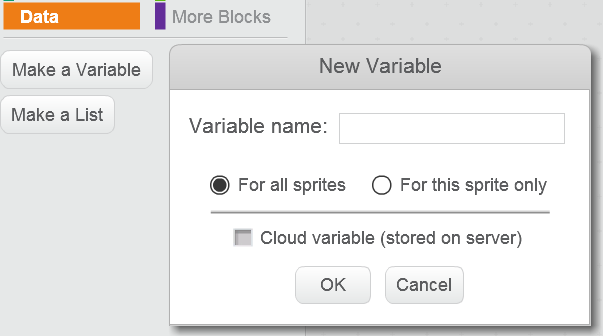
\includegraphics[width=\columnwidth]{fig/ui-vars.png}
  \caption{The Scratch user interface to create a variable}
  \label{fig:ui-vars}
  \end{center}
\end{figure} 

\subsection{Procedures}
Scratch also allows users to create their own blocks, called procedures. They can have input parameters, and labels in between them. Functions are created with an interface similar to the one to create variables. Figure \ref{fig:functions} shows the definition and invocation of a procedure.

\begin{figure}
  \begin{center}
  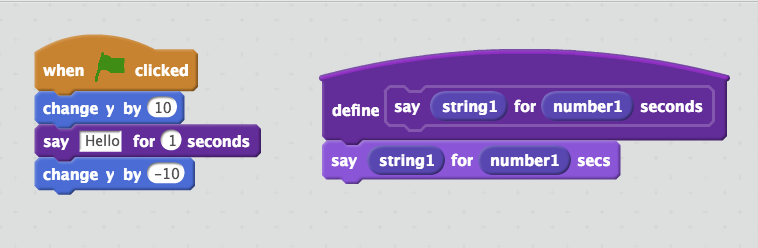
\includegraphics[width=\columnwidth]{fig/functions.png}
  \caption{Scratch code to define and invoke a procedure}
  \label{fig:functions}
  \end{center}
\end{figure} 


\section{Research design and dataset}
\subsection{Overall design}
\todo{here we need to tell something about replications, see the paper by Shull et al on importance of replications in software engineering.}

\subsection{Dataset}


\subsection{Data analysis}
To augment the visual comparison of the variable name data derived from Scratch as well as the programming languages considered by Beniamini et al.~\cite{Beniamini}, we conduct statistical analysis. 

Understanding differences in variable name lengths requires comparison of multiple distributions, traditionally performed as a two-step process consisting of (1) testing a global null hypothesis, that can be intuitively formulated as ``all distributions are the same'', using ANOVA or its non-parametric counterpart, the Kruskal-Wallis test, and (2) performing multiple pairwise comparisons of different distributions, testing specific subhypotheses such as ``distributions 2 and 4 are the same''. 
However, it has been observed that such a two-step approach can result in inconsistencies when either the global null hypothesis is rejected but none of the pairwise subhypotheses is rejected or vice versa~\cite{Gabriel}. 
Moreover, it has been suggested that the Wilcoxon-Mann-Whitney test, commonly used for subhypothesis testing, is not robust to unequal population variances, especially in the unequal sample size case~\cite{Zimmerman:Zumbo}
Therefore, one-step approaches have been sought.
We opt for one such approach, the $\widetilde{\mathbf{T}}$-procedure of Konietschke et al.~\cite{Konietschke:Hothorn:Brunner}. 
This procedure is robust against unequal population variances, respects transitivity, and has been successfully applied in empirical software engineering~\cite{VasilescuSGM14,VasilescuCS14,YuWYW16}.
In particular, we use the Tukey (all-pairs) contrasts to compare all distributions pairwise.

Furthermore, to understand differences and similarities between the distributions of single-letter variable names in different languages we represent each programming language as a 26-dimensional vector with the dimensions corresponding to `a', ..., `z', and apply hierarchical clustering. \todo{why hierarchical?}
 \section{Results}

Figure \ref{fig:distribution_of_lengths} shows the distribution of lengths in the corpus.

\begin{figure}[h]
	\begin{center}
		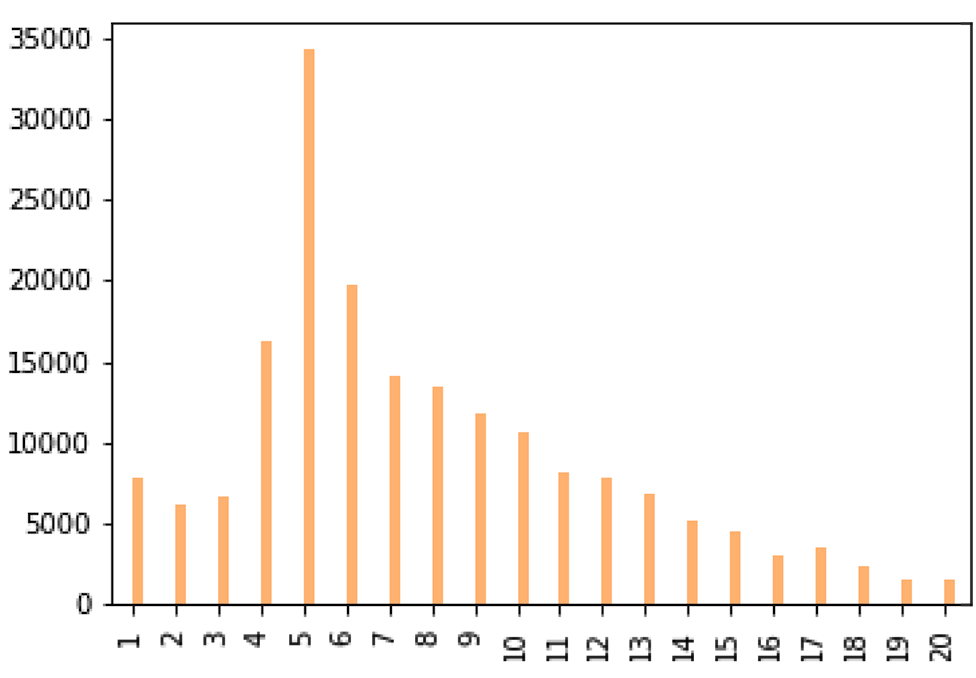
\includegraphics[width=\columnwidth]{fig/distribution_of_lengths}
		\caption{Total occurrence of variables of different lengths}
		\label{fig:distribution_of_lengths}
	\end{center}
\end{figure} 

\todo{we could sample some 5 letter identifiers here to see what they usually look like since they are an interesting peak?}

\todo{in the ICPC paper the diagram goes to 20 and then just has 20+ we could do that too?}
\subsection{One letters}

Figure \ref{fig:one_letter_occurrence} shows the distribution of variables of one letter in the corpus.

\begin{figure}[h]
	\begin{center}
		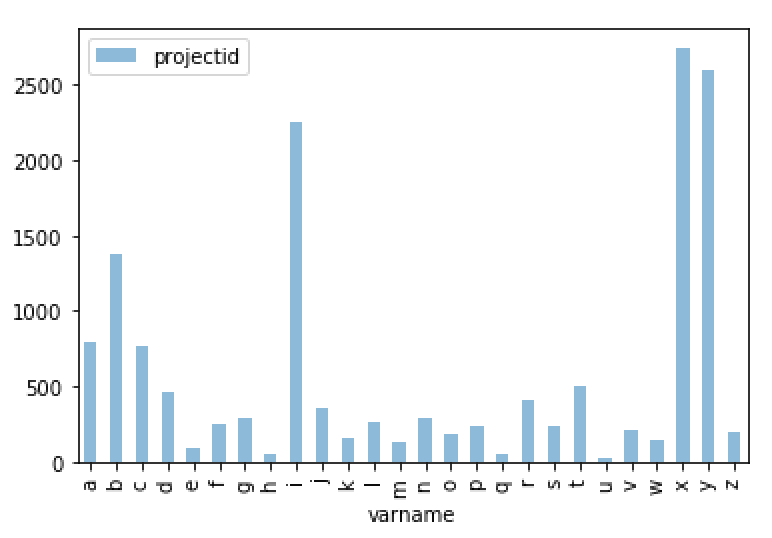
\includegraphics[width=\columnwidth]{fig/one_letter_occurrence}
		\caption{Total occurrence of variables of one letter}
		\label{fig:one_letter_occurrence}
	\end{center}
\end{figure} 


Figure \ref{fig:one_letter_occurrence_functions} shows the distribution of \emph{functions} of one letter in the corpus.

\begin{figure}[h]
	\begin{center}
		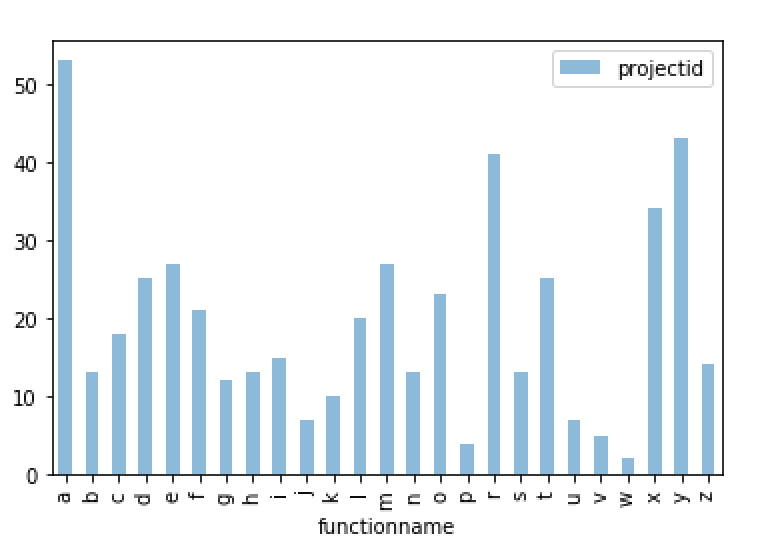
\includegraphics[width=\columnwidth]{fig/one_letter_occurrence_functions}
		\caption{Total occurrence of functions of one letter}
		\label{fig:one_letter_occurrence_functions}
	\end{center}
\end{figure} 

Scratch is not a typed language, variables can contain strings or numbers without declarations or casting. However, we can infer the types by attempting to cast them to a float or an int. As such we did obtain types, allowing us to compare to the ICPC paper.

Figure \ref{fig:one_letter_type} shows the distribution of variables of one letter in the corpus.

\todo{here we can reflect on the differences with "real" languages and the prevalence of ints.}

\begin{figure}
	\begin{center}
		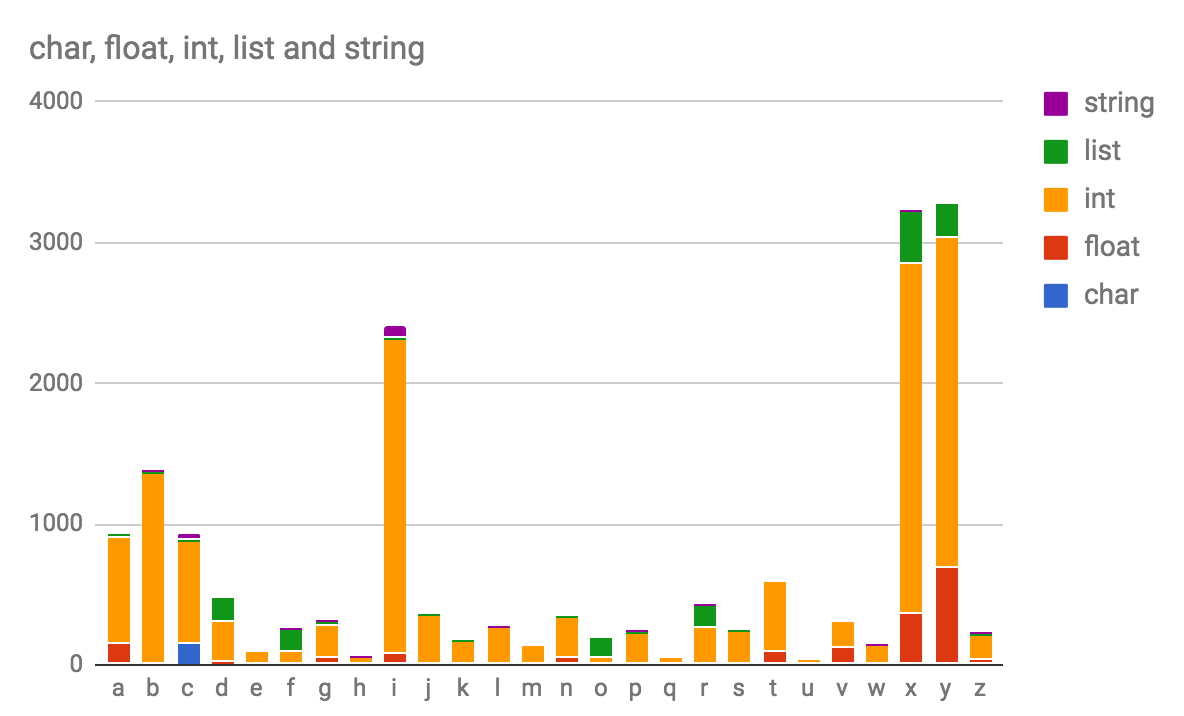
\includegraphics[width=\columnwidth]{fig/one_letter_type}
		\caption{Inferred types for variables of one letter}
		\label{fig:one_letter_type}
	\end{center}
\end{figure} 

\subsection{Use of spaces in variable names}

Contrary to most textual programming languages, Scratch allows users to use spaces in variable names. This is quite commonly used, about 30.000 projects use one or more variables with a space in it, versus 60.000 that use only space-free variable names. Figure \ref{fig:number_of_spaces} shows the distribution of spaces in variable names. We have found that many introductory Scratch programming materials demonstrate the use of space free variables, and that children---and adults---that already have programming experience deem the use of spaces in variables as non-natural, even though arguable `number of apples' is more natural that `nApples'.

\begin{figure}
	\begin{center}
		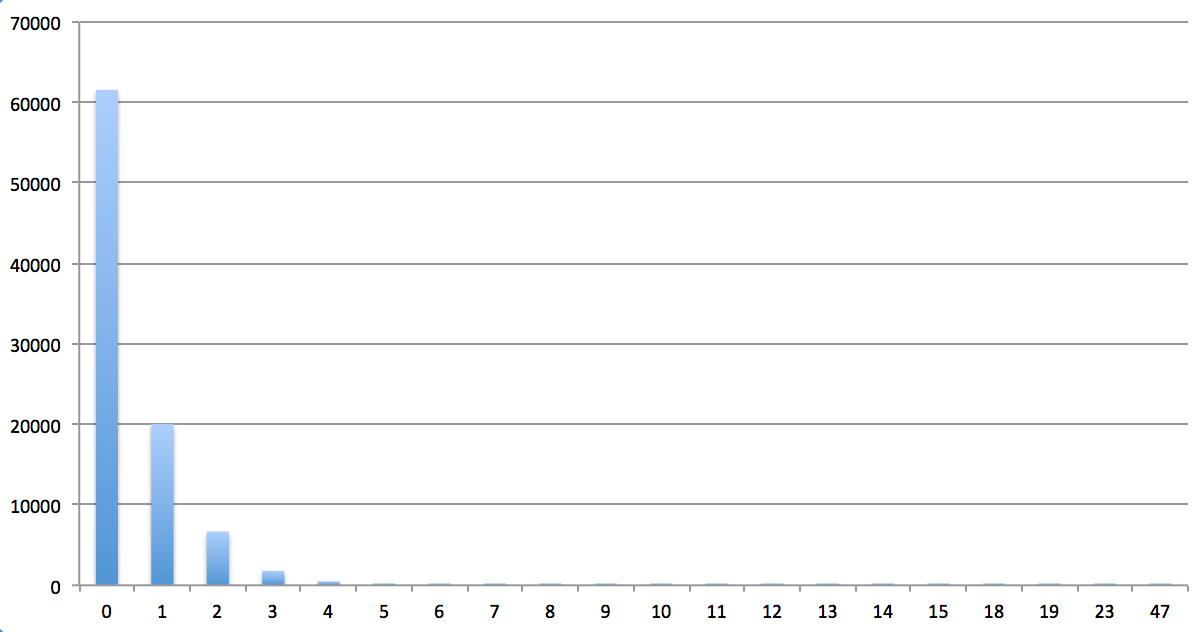
\includegraphics[width=\columnwidth]{fig/number_of_spaces}
		\caption{Number of spaces in variable names}
		\label{fig:number_of_spaces}
	\end{center}
\end{figure} 

\subsection{Use of non-letter variable names}
In addition to spaces in variable names, Scratch even allows the use of numbers and even floating point numbers as variables. We found 718 projects with integer variable names and 19 with floating point names. While their use is rare, we manually examined some projects and numbers are used in interesting and clever ways.

\todo{here we can show the tic tac toe example}

 \section{Discussion}
 \section{Conclusions}

\section{Conclusion}
The conclusion goes here.




% conference papers do not normally have an appendix


% use section* for acknowledgment
\section*{Acknowledgment}


The authors would like to thank...





% trigger a \newpage just before the given reference
% number - used to balance the columns on the last page
% adjust value as needed - may need to be readjusted if
% the document is modified later
%\IEEEtriggeratref{8}
% The "triggered" command can be changed if desired:
%\IEEEtriggercmd{\enlargethispage{-5in}}

% references section

% can use a bibliography generated by BibTeX as a .bbl file
% BibTeX documentation can be easily obtained at:
% http://mirror.ctan.org/biblio/bibtex/contrib/doc/
% The IEEEtran BibTeX style support page is at:
% http://www.michaelshell.org/tex/ieeetran/bibtex/
\bibliographystyle{IEEEtran}
% argument is your BibTeX string definitions and bibliography database(s)
\bibliography{paper}
%
% <OR> manually copy in the resultant .bbl file
% set second argument of \begin to the number of references
% (used to reserve space for the reference number labels box)

% that's all folks
\end{document}


